% hfg_weyl_correspondence.tex
% Standalone TikZ figure: the factor-by-factor Weyl-group correspondence
% for the 576-element Galois closure (CLAIMS_REGISTER.md entry 15).
% Compile with: pdflatex hfg_weyl_correspondence.tex
\documentclass[tikz,border=8pt]{standalone}
\usepackage{amsmath,amssymb}
\usetikzlibrary{arrows.meta,positioning}

\definecolor{hfggreen}{HTML}{2A5E2A}
\definecolor{hfgtan}{HTML}{7B5A2E}

\begin{document}
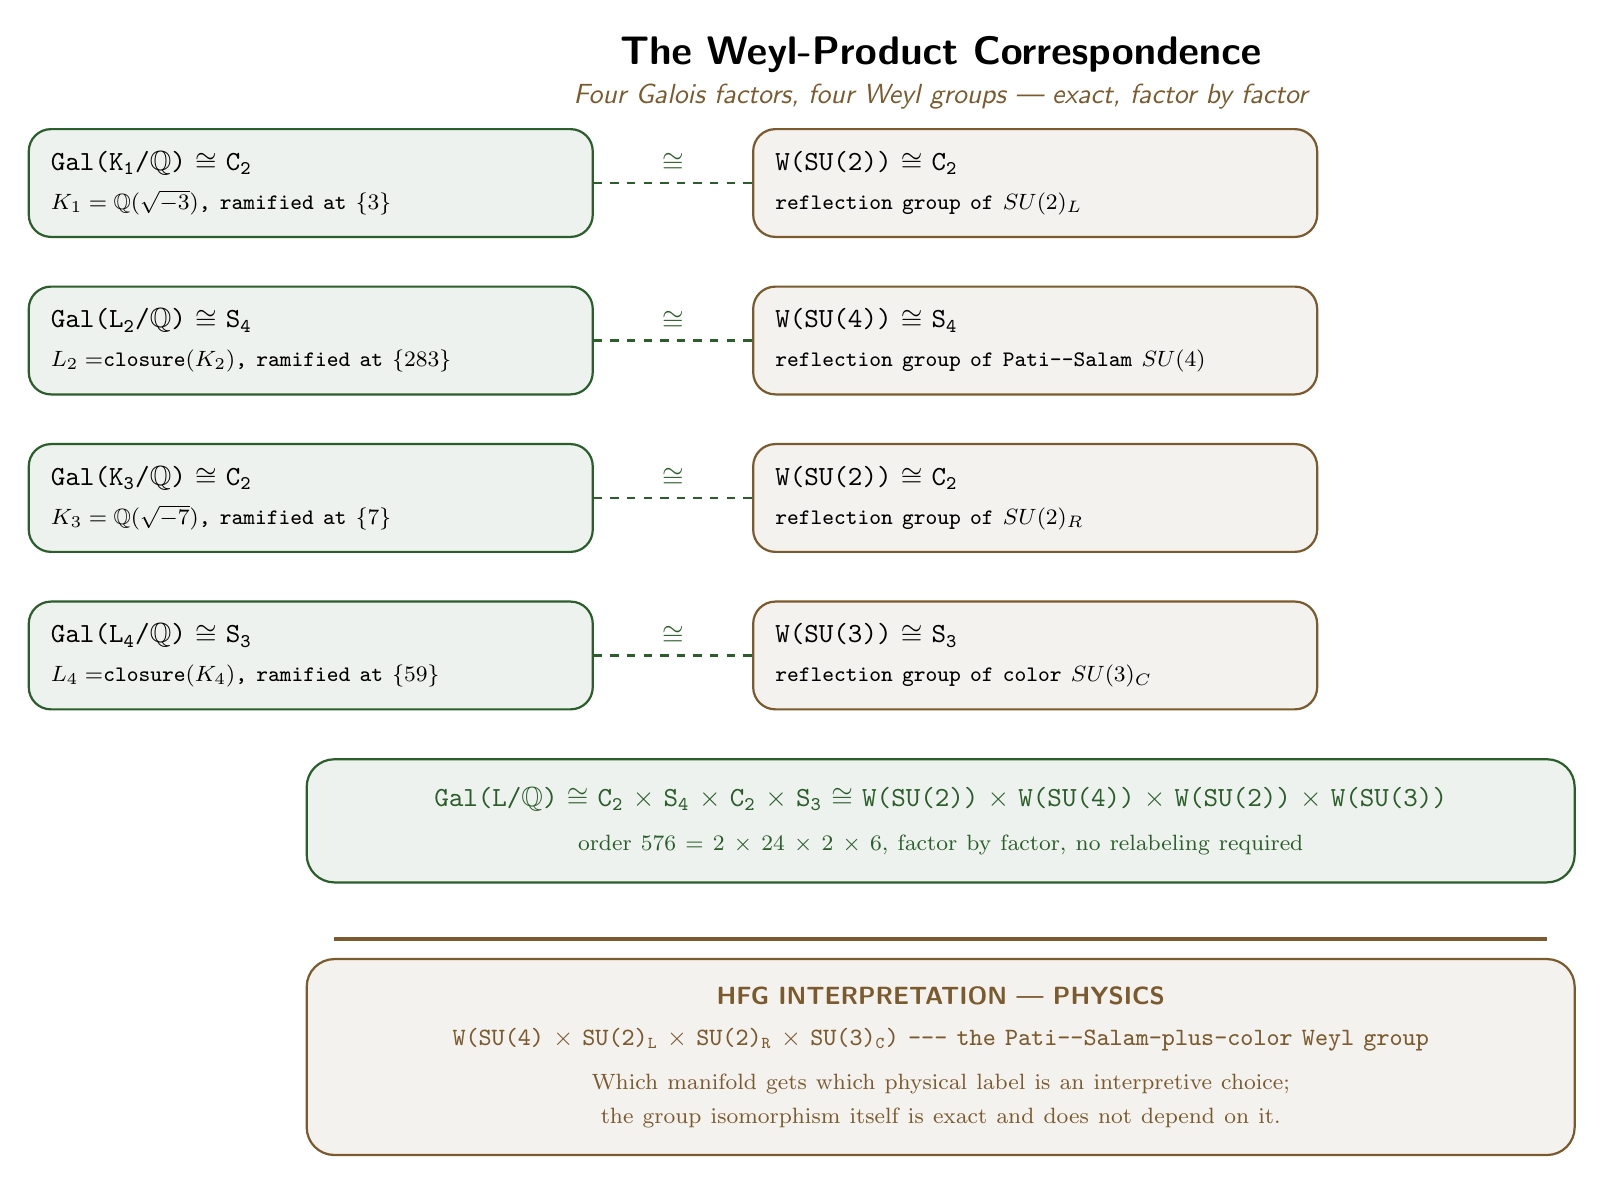
\begin{tikzpicture}[
  font=\sffamily,
  algebra/.style={rounded corners=8pt, draw=hfggreen, fill=hfggreen!8, thick, align=left, text width=6.6cm, inner sep=8pt},
  physical/.style={rounded corners=8pt, draw=hfgtan, fill=hfgtan!8, thick, align=left, text width=6.6cm, inner sep=8pt},
  result/.style={rounded corners=10pt, draw=hfggreen, fill=hfggreen!8, thick, align=center, text width=15.4cm, inner sep=10pt},
  interp/.style={rounded corners=10pt, draw=hfgtan, fill=hfgtan!8, thick, align=center, text width=15.4cm, inner sep=10pt},
  link/.style={hfggreen, dashed, thick}
]

\node[align=center] at (8,10.4) {\Large\bfseries The Weyl-Product Correspondence\\[2pt]
  \normalsize\itshape\color{hfgtan} Four Galois factors, four Weyl groups --- exact, factor by factor};

\node[algebra] (r1a) at (0,9.0)  {\ttfamily Gal(K\textsubscript{1}/$\mathbb{Q}$) $\cong$ C\textsubscript{2}\\[2pt]\footnotesize $K_1=\mathbb{Q}(\sqrt{-3})$, ramified at $\{3\}$};
\node[physical] (r1b) at (9.2,9.0) {\ttfamily W(SU(2)) $\cong$ C\textsubscript{2}\\[2pt]\footnotesize reflection group of $SU(2)_L$};
\draw[link] (r1a.east) -- (r1b.west) node[midway,above,hfggreen]{$\cong$};

\node[algebra] (r2a) at (0,7.0)  {\ttfamily Gal(L\textsubscript{2}/$\mathbb{Q}$) $\cong$ S\textsubscript{4}\\[2pt]\footnotesize $L_2=$closure$(K_2)$, ramified at $\{283\}$};
\node[physical] (r2b) at (9.2,7.0) {\ttfamily W(SU(4)) $\cong$ S\textsubscript{4}\\[2pt]\footnotesize reflection group of Pati--Salam $SU(4)$};
\draw[link] (r2a.east) -- (r2b.west) node[midway,above,hfggreen]{$\cong$};

\node[algebra] (r3a) at (0,5.0)  {\ttfamily Gal(K\textsubscript{3}/$\mathbb{Q}$) $\cong$ C\textsubscript{2}\\[2pt]\footnotesize $K_3=\mathbb{Q}(\sqrt{-7})$, ramified at $\{7\}$};
\node[physical] (r3b) at (9.2,5.0) {\ttfamily W(SU(2)) $\cong$ C\textsubscript{2}\\[2pt]\footnotesize reflection group of $SU(2)_R$};
\draw[link] (r3a.east) -- (r3b.west) node[midway,above,hfggreen]{$\cong$};

\node[algebra] (r4a) at (0,3.0)  {\ttfamily Gal(L\textsubscript{4}/$\mathbb{Q}$) $\cong$ S\textsubscript{3}\\[2pt]\footnotesize $L_4=$closure$(K_4)$, ramified at $\{59\}$};
\node[physical] (r4b) at (9.2,3.0) {\ttfamily W(SU(3)) $\cong$ S\textsubscript{3}\\[2pt]\footnotesize reflection group of color $SU(3)_C$};
\draw[link] (r4a.east) -- (r4b.west) node[midway,above,hfggreen]{$\cong$};

\node[result] (combined) at (8,0.9) {
  \ttfamily\color{hfggreen} Gal(L/$\mathbb{Q}$) $\cong$ C\textsubscript{2} $\times$ S\textsubscript{4} $\times$ C\textsubscript{2} $\times$ S\textsubscript{3}
  $\cong$ W(SU(2)) $\times$ W(SU(4)) $\times$ W(SU(2)) $\times$ W(SU(3))\\[4pt]
  \normalfont\footnotesize order 576 = 2 $\times$ 24 $\times$ 2 $\times$ 6, factor by factor, no relabeling required
};

\draw[hfgtan, very thick] (0.3,-0.6) -- (15.7,-0.6);
\node[hfgtan, font=\itshape\small] at (8,-1.0) {THE PROVED ALGEBRA ENDS ABOVE THIS LINE};

\node[interp] (interp) at (8,-2.1) {
  \small\bfseries\color{hfgtan} HFG INTERPRETATION --- PHYSICS\\[4pt]
  \normalfont\ttfamily W(SU(4) $\times$ SU(2)\textsubscript{L} $\times$ SU(2)\textsubscript{R} $\times$ SU(3)\textsubscript{C}) --- the Pati--Salam-plus-color Weyl group\\[4pt]
  \normalfont\footnotesize Which manifold gets which physical label is an interpretive choice; the group isomorphism itself is exact and does not depend on it.
};

\end{tikzpicture}
\end{document}
